% Options for packages loaded elsewhere
\PassOptionsToPackage{unicode}{hyperref}
\PassOptionsToPackage{hyphens}{url}
\PassOptionsToPackage{dvipsnames,svgnames,x11names}{xcolor}
\documentclass[
  10pt,
  fontset=fandol]{ctexart}
\usepackage{xcolor}
\usepackage[margin=16mm]{geometry}
\usepackage{amsmath,amssymb}
\setcounter{secnumdepth}{-\maxdimen} % remove section numbering
\usepackage{iftex}
\ifPDFTeX
  \usepackage[T1]{fontenc}
  \usepackage[utf8]{inputenc}
  \usepackage{textcomp} % provide euro and other symbols
\else % if luatex or xetex
  \usepackage{unicode-math} % this also loads fontspec
  \defaultfontfeatures{Scale=MatchLowercase}
  \defaultfontfeatures[\rmfamily]{Ligatures=TeX,Scale=1}
\fi
\usepackage{lmodern}
\ifPDFTeX\else
  % xetex/luatex font selection
\fi
% Use upquote if available, for straight quotes in verbatim environments
\IfFileExists{upquote.sty}{\usepackage{upquote}}{}
\IfFileExists{microtype.sty}{% use microtype if available
  \usepackage[]{microtype}
  \UseMicrotypeSet[protrusion]{basicmath} % disable protrusion for tt fonts
}{}
\makeatletter
\@ifundefined{KOMAClassName}{% if non-KOMA class
  \IfFileExists{parskip.sty}{%
    \usepackage{parskip}
  }{% else
    \setlength{\parindent}{0pt}
    \setlength{\parskip}{6pt plus 2pt minus 1pt}}
}{% if KOMA class
  \KOMAoptions{parskip=half}}
\makeatother
\usepackage{graphicx}
\makeatletter
\newsavebox\pandoc@box
\newcommand*\pandocbounded[1]{% scales image to fit in text height/width
  \sbox\pandoc@box{#1}%
  \Gscale@div\@tempa{\textheight}{\dimexpr\ht\pandoc@box+\dp\pandoc@box\relax}%
  \Gscale@div\@tempb{\linewidth}{\wd\pandoc@box}%
  \ifdim\@tempb\p@<\@tempa\p@\let\@tempa\@tempb\fi% select the smaller of both
  \ifdim\@tempa\p@<\p@\scalebox{\@tempa}{\usebox\pandoc@box}%
  \else\usebox{\pandoc@box}%
  \fi%
}
% Set default figure placement to htbp
\def\fps@figure{htbp}
\makeatother
\setlength{\emergencystretch}{3em} % prevent overfull lines
\providecommand{\tightlist}{%
  \setlength{\itemsep}{0pt}\setlength{\parskip}{0pt}}
\usepackage{amsmath,amssymb,mathtools,needspace}
\xeCJKDeclareCharClass{CJK}{"2032,"0400->"04FF,"2160->"216B,"2460->"2473,"25A0,"25C7,"25CB,"25CF}
\IfFontExistsTF{Arial Unicode MS}{\xeCJKsetup{AutoFallBack=true}\setCJKfallbackfamilyfont{\CJKrmdefault}{Arial Unicode MS}}{}
\setcounter{secnumdepth}{0}
\setlength{\emergencystretch}{2em}
\allowdisplaybreaks
\usepackage{bookmark}
\IfFileExists{xurl.sty}{\usepackage{xurl}}{} % add URL line breaks if available
\urlstyle{same}
\hypersetup{
  pdftitle={FWT 的计算流程},
  colorlinks=true,
  linkcolor={Maroon},
  filecolor={Maroon},
  citecolor={Blue},
  urlcolor={Blue},
  pdfcreator={LaTeX via pandoc}}

\title{FWT 的计算流程}
\author{}
\date{}

\begin{document}
\maketitle

\subsubsection{10.4.3　FWT 的计算流程}\label{fwt-ux7684ux8ba1ux7b97ux6d41ux7a0b}

二分手续（10.4.2）采取两两加工的处理方式，即将一对数据 \((x(j),x(N/2+j))\) 加工成一对新的数据 \((x_1(j),x_1(N/2+j))\)，其计算格式如图 10.6 所示。这里分别用实线与虚线区分数据的相加与相减两种运算。

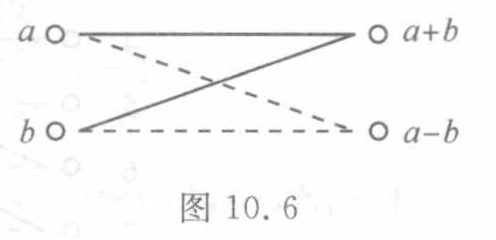
\includegraphics[width=0.85\linewidth,height=\textheight,keepaspectratio,alt={图 10.6（原图裁切）：两两加工的计算格式}]{../assets/ch10/fig-10-6.png}

图 10.6

\begin{quote}
图中文字与图意（转录）：左端输入从上到下为 \(a\)、\(b\)，右端输出从上到下为 \(a+b\)、\(a-b\)。输入至上方输出的两条线为实线，输入至下方输出的两条线为虚线，形成交叉的两两计算格式。
\end{quote}

现在运用二分技术针对 8-WT：

\[
X(i)=\sum_{j=0}^{7}x(j)H_8(i,j),\quad i=0,1,\cdots,7.
\tag{10.4.3}
\]

具体显示前述 FWT 的计算流程。

\textbf{步 1}　施行 \(N=8\) 的二分手续（10.4.2），即

\[
x_1(0)=x(0)+x(4),\quad x_1(4)=x(0)-x(4),
\]

\begin{quote}
校注（agent 补充）：原页``使问题的的规模减半''重复``的''，上文照录。
\end{quote}

\href{../../source-images/pdf-273.jpeg}{原页}

\[
\begin{aligned}
x_1(1)&=x(1)+x(5),& x_1(5)&=x(1)-x(5),\\
x_1(2)&=x(2)+x(6),& x_1(6)&=x(2)-x(6),\\
x_1(3)&=x(3)+x(7),& x_1(7)&=x(3)-x(7),
\end{aligned}
\]

将所给 8-WT 加工成 2 个 4-WT。借助于图 10.6 的计算格式，这一演化步骤如图 10.7 所示。

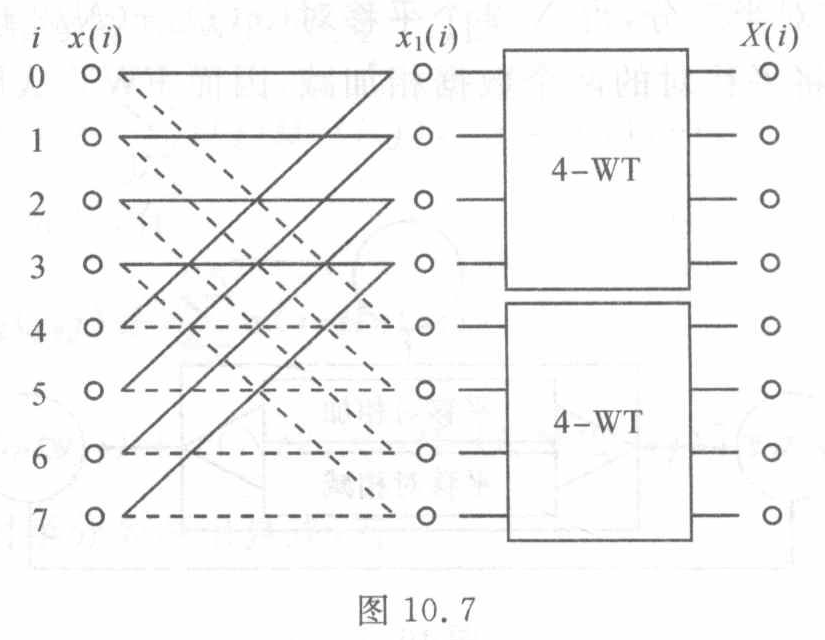
\includegraphics[width=0.85\linewidth,height=\textheight,keepaspectratio,alt={图 10.7（原图裁切）：8-WT 经第一步化成两个 4-WT}]{../assets/ch10/fig-10-7.png}

图 10.7

\begin{quote}
图中文字与图意（转录）：从左到右的列标为 \(i\)、\(x(i)\)、\(x_1(i)\)、\(X(i)\)。\(i\) 的行标为 0、1、2、3、4、5、6、7；两组模块均标为 4-WT。第一个加工阶段将行对 \((0,4)\)、\((1,5)\)、\((2,6)\)、\((3,7)\) 相加减，所得 \(x_1(i)\) 的前四项、后四项分别接入一个 4-WT，右端输出 \(X(i)\)。
\end{quote}

\textbf{步 2}　对 2 个 4-WT 分别施行 \(N=4\) 的二分手续（10.4.2），即

\[
\begin{aligned}
x_2(0)&=x_1(0)+x_1(2),& x_2(2)&=x_1(0)-x_1(2),\\
x_2(1)&=x_1(1)+x_1(3),& x_2(3)&=x_1(1)-x_1(3)
\end{aligned}
\]

与

\[
\begin{aligned}
x_2(4)&=x_1(4)+x_1(6),& x_2(6)&=x_1(4)-x_1(6),\\
x_2(5)&=x_1(5)+x_1(7),& x_2(7)&=x_1(5)-x_1(7),
\end{aligned}
\]

进一步加工出关于数据 \(\{x_2(j)\}\) 的 4 个 2-WT。这一演化步如图 10.8 所示。

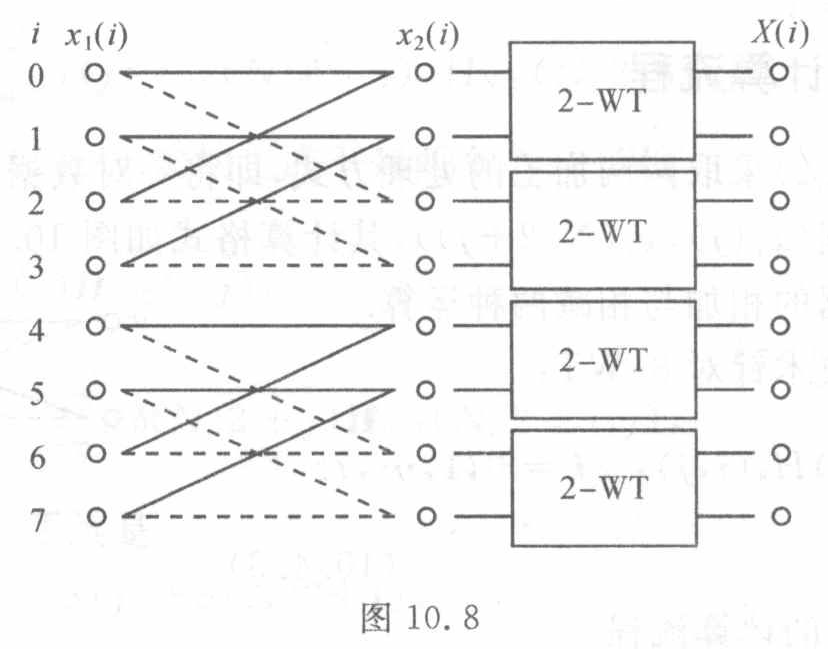
\includegraphics[width=0.85\linewidth,height=\textheight,keepaspectratio,alt={图 10.8（原图裁切）：两个 4-WT 经第二步化成四个 2-WT}]{../assets/ch10/fig-10-8.png}

图 10.8

\begin{quote}
图中文字与图意（转录）：从左到右的列标为 \(i\)、\(x_1(i)\)、\(x_2(i)\)、\(X(i)\)。\(i\) 的行标为 0、1、2、3、4、5、6、7；四组模块均标为 2-WT。该阶段将行对 \((0,2)\)、\((1,3)\)、\((4,6)\)、\((5,7)\) 相加减，所得 \(x_2(i)\) 每两项接入一个 2-WT，右端输出 \(X(i)\)。
\end{quote}

\textbf{步 3}　再对每个 2-WT 分别施行二分手续，即

\href{../../source-images/pdf-274.jpeg}{原页}

\[
\begin{aligned}
x_3(0)&=x_2(0)+x_2(1),& x_3(1)&=x_2(0)-x_2(1),\\
x_3(2)&=x_2(2)+x_2(3),& x_3(3)&=x_2(2)-x_2(3),\\
x_3(4)&=x_2(4)+x_2(5),& x_3(5)&=x_2(4)-x_2(5),\\
x_3(6)&=x_2(6)+x_2(7),& x_3(7)&=x_2(6)-x_2(7).
\end{aligned}
\]

加工得出关于数据 \(\{x_3(i)\}\) 的 8 个 1-WT，即得所求结果：

\[
X(i)=x_3(i),\quad i=0,1,\cdots,7.
\]

上述算法 FWT，其计算模型与输入数据同步进行加工，在将计算模型从 8-WT 加工成 1-WT 的同时，输入数据被加工成输出结果 \(\{X(i)\}\)。综合上述各步即得 FWT 的数据加工流程图 10.9。

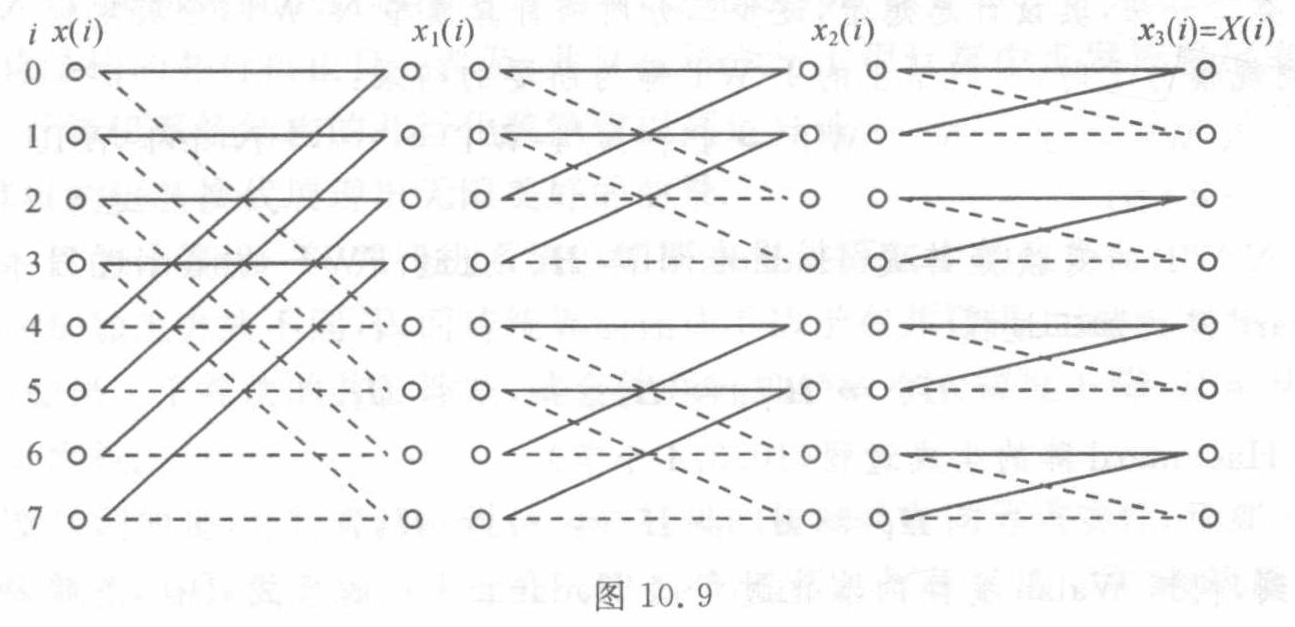
\includegraphics[width=0.85\linewidth,height=\textheight,keepaspectratio,alt={图 10.9（原图裁切）：8-WT 的完整数据加工流程}]{../assets/ch10/fig-10-9.png}

图 10.9

\begin{quote}
图中文字与图意（转录）：列标依次为 \(i\)、\(x(i)\)、\(x_1(i)\)、\(x_2(i)\)、\(x_3(i)=X(i)\)，行标为 0、1、2、3、4、5、6、7。第一阶段配对 \((0,4)\)、\((1,5)\)、\((2,6)\)、\((3,7)\)；第二阶段配对 \((0,2)\)、\((1,3)\)、\((4,6)\)、\((5,7)\)；第三阶段配对 \((0,1)\)、\((2,3)\)、\((4,5)\)、\((6,7)\)。每对按图 10.6 的实线相加、虚线相减计算，三步后由 \(x_3(i)\) 得到 \(X(i)\)。
\end{quote}

\begin{center}\rule{0.5\linewidth}{0.5pt}\end{center}

\subsection{相关原页校注（agent 补充）}\label{ux76f8ux5173ux539fux9875ux6821ux6ce8agent-ux8865ux5145}

以下校注来自本节覆盖的原页，可能也涉及同页相邻小节；原文照录与校正说明分开保留。

\subsubsection{原书 PDF 页 274 的校注}\label{ux539fux4e66-pdf-ux9875-274-ux7684ux6821ux6ce8}

\href{../pages/pdf-274.md}{完整原页转录} · \href{../../source-images/pdf-274.jpeg}{原页图像}

校注记录：CH10-E004。

\begin{quote}
校注（agent 补充，CH10-E004）：式（10.4.4）原印 \(l=1,2,\cdots,2^k\)，上文照录。此式用 \((l-1)N_{k-1}\) 定位第 \(k-1\) 步的数据段，该步只有 \(2^{k-1}\) 段，因此上限应为 \(2^{k-1}\)。例如 \(N=8,k=1\) 时，按原印取 \(l=2\) 会访问从索引 8 开始的数据，越过 \(0,\ldots,7\)。本页前文用于描述第 \(k\) 步结果分段数的 \(2^k\) 则正确。下一页算法 10.1 引用此式，也受该范围疑误影响。\href{../assets/ch10/erratum-p274-range.png}{原式放大裁片}。
\end{quote}

\subsection{本节覆盖原页的校注记录}\label{ux672cux8282ux8986ux76d6ux539fux9875ux7684ux6821ux6ce8ux8bb0ux5f55}

下列记录按原页关联，含同页相邻小节的校注；计算时同时读取上文校注和完整原页。

\begin{itemize}
\tightlist
\item
  \texttt{CH10-E003}：原书 PDF 页 272
\item
  \texttt{CH10-E004}：原书 PDF 页 274
\end{itemize}

\end{document}
